\label{chap:circuit}

Nội dung cụ thể của chương 2
sẽ triển khai các cơ sở toán học thành mô hình tính toán lượng tử cụ thể. Mục~\ref{sec:qubit}
xây dựng khái niệm qubit -- đơn vị thông tin cơ bản -- từ trạng thái đơn lẻ đến hệ
nhiều qubit. Mục 2.2 khảo sát các cổng lượng tử phổ biến như các biểu
hiện rời rạc của tiên đề tiến hóa. Mục 2.3 trình bày cấu trúc
mạch và phép đo -- đủ để đọc hiểu và triển khai thuật toán Deutsch--Jozsa ở
Chương 3. Nội dung của chương được tham khảo chính từ giáo trình kinh điển của Nielsen \& Chuang~\cite{ref5} và các tài liệu của Maassen~\cite{ref4} và Kuperberg~\cite{ref3}.

% ================================================================
\section{Qubit: biểu diễn toán học và hình học Bloch}
\label{sec:qubit}

% ---------------------------------------------------------------
\subsection*{Trạng thái qubit và ràng buộc chuẩn hóa}

Trong lý thuyết thông tin lượng tử, đơn vị thông tin cơ bản là \textbf{qubit}
(\textit{quantum bit}) là một hệ lượng tử hai mức được mô tả bởi một vectơ đơn
vị trong không gian Hilbert phức hai chiều $\mathbb{C}^2$ \cite{ref5}. Khác với
bit cổ điển chỉ nhận một trong hai giá trị xác định $0$ hoặc $1$, qubit có thể
tồn tại trong vô số trạng thái trung gian -- gọi là \textbf{trạng thái chồng chất}
-- tạo nên nền tảng cho sức mạnh tính toán của máy tính lượng tử.

Hai trạng thái cơ sở trực chuẩn của $\mathbb{C}^2$ được ký hiệu là $|0\rangle$
và $|1\rangle$ theo ký hiệu Dirac, tương ứng với hai
giá trị cổ điển $0$ và $1$, và tạo thành \textbf{cơ sở tính toán}
(\textit{computational basis}). Trong biểu diễn vectơ cột:
$$|0\rangle = \begin{pmatrix}1\\0\end{pmatrix}, \qquad
  |1\rangle = \begin{pmatrix}0\\1\end{pmatrix}.$$

Theo nguyên lý chồng chất (hệ quả của Tiên đề~1, mục~\ref{sec:postulates}),
trạng thái tổng quát của một qubit là \cite{ref5}:
\begin{equation}
    |\psi\rangle = \alpha|0\rangle + \beta|1\rangle,
    \quad \alpha,\beta \in \mathbb{C},
    \label{eq:qubit}
\end{equation}
trong đó $\alpha$ và $\beta$ được gọi là các \textbf{biên độ xác suất}. Khi thực
hiện phép đo trong cơ sở tính toán, hệ suy sụp về $|0\rangle$ với xác suất
$|\alpha|^2$ và về $|1\rangle$ với xác suất $|\beta|^2$. Điều kiện chuẩn hóa
$\langle\psi|\psi\rangle = 1$ (Tiên đề~1) đòi hỏi:
\begin{equation}
    |\alpha|^2 + |\beta|^2 = 1.
    \label{eq:normalization}
\end{equation}

Vì $\alpha, \beta \in \mathbb{C}$ là các số phức, mỗi biên độ có thể viết dưới
dạng Euler $\alpha = |\alpha|e^{i\gamma_\alpha}$ và
$\beta = |\beta|e^{i\gamma_\beta}$, trong đó $|\alpha|, |\beta| \geq 0$ là độ
lớn và $\gamma_\alpha, \gamma_\beta \in \mathbb{R}$ là các góc pha
(xem Phụ lục 3 để hiểu cách biểu diễn số phức dạng Euler).
Khi đó trạng thái qubit~\eqref{eq:qubit} có thể tách thành:
$$|\psi\rangle
= e^{i\gamma_\alpha}\!\left(|\alpha|\,|0\rangle
+ |\beta|\,e^{i(\gamma_\beta - \gamma_\alpha)}|1\rangle\right).$$
Biểu thức này cho thấy hai loại pha có vai trò vật lý hoàn toàn khác nhau.

\begin{definition}[Pha toàn cục và pha tương đối]
\label{def:phase}
Cho trạng thái qubit $|\psi\rangle = \alpha|0\rangle + \beta|1\rangle$ với
$\alpha = |\alpha|e^{i\gamma_\alpha}$, $\beta = |\beta|e^{i\gamma_\beta}$.
\begin{enumerate}[label=(\roman*)]
    \item \textbf{Pha toàn cục} là hệ số $e^{i\gamma_\alpha}$ nhân vào toàn bộ
          trạng thái -- tức hệ số đứng \emph{ngoài} toàn bộ biểu thức.
    \item \textbf{Pha tương đối} là $e^{i(\gamma_\beta - \gamma_\alpha)}$ --
          hệ số lệch pha \emph{giữa} biên độ của $|1\rangle$ so với $|0\rangle$.
\end{enumerate}
\end{definition}

\begin{remark}
Pha toàn cục \emph{không có ý nghĩa vật lý quan sát được}. Thật vậy, vì
$|e^{i\gamma}| = 1$ với mọi $\gamma \in \mathbb{R}$, mọi xác suất đo lường đều
không thay đổi khi nhân thêm pha toàn cục:
$$|\langle\phi\,|\,e^{i\gamma}\psi\rangle|^2
= |e^{i\gamma}|^2\,|\langle\phi|\psi\rangle|^2
= |\langle\phi|\psi\rangle|^2.$$
Do đó $|\psi\rangle$ và $e^{i\gamma}|\psi\rangle$ là tương đương về mặt vật lý.

Ngược lại, pha tương đối \emph{có thể quan sát được} thông qua giao thoa. Ví dụ,
hai trạng thái
$$|{+}\rangle = \frac{|0\rangle + |1\rangle}{\sqrt{2}}, \qquad
  |{-}\rangle = \frac{|0\rangle - |1\rangle}{\sqrt{2}}$$
có cùng xác suất $1/2$ khi đo trong cơ sở tính toán $\{|0\rangle, |1\rangle\}$,
nhưng khác nhau ở pha tương đối: $|+\rangle$ có pha tương đối $0$ (cùng dấu),
còn $|-\rangle$ có pha tương đối $\pi$ (ngược dấu). Sự khác biệt này bộc lộ rõ
khi đo trong cơ sở Hadamard $\{|+\rangle, |-\rangle\}$:
$$|\langle{+}|{+}\rangle|^2 = 1, \quad |\langle{-}|{+}\rangle|^2 = 0, \qquad
  |\langle{+}|{-}\rangle|^2 = 0, \quad |\langle{-}|{-}\rangle|^2 = 1.$$
Hai trạng thái hoàn toàn phân biệt nhau -- dù không thể phân biệt nếu chỉ đo
trong cơ sở tính toán. 
\end{remark}

% ---------------------------------------------------------------
\subsection*{Mặt cầu Bloch}

Điều kiện chuẩn hóa ở phương trình~\eqref{eq:normalization} cùng với việc loại bỏ pha toàn
cục cho phép xây dựng một biểu diễn hình học trực quan cho trạng thái qubit.
Cụ thể, mọi trạng thái thuần khiết của một qubit được tham số hóa duy nhất qua
hai góc thực $\theta \in [0,\pi]$ và $\phi \in [0,2\pi)$ \cite{ref5}:
\begin{equation}
    |\psi\rangle = \cos\frac{\theta}{2}|0\rangle
                + e^{i\phi}\sin\frac{\theta}{2}|1\rangle.
    \label{eq:bloch-param}
\end{equation}
Để nắm rõ hơn về nguồn gốc của phương trình~\eqref{eq:bloch-param} ta xem Phụ lục 4. Cặp $(\theta, \phi)$ xác định một điểm trên mặt cầu đơn vị trong $\mathbb{R}^3$
thông qua tọa độ Descartes:
$$\vec{r} = (\sin\theta\cos\phi,\; \sin\theta\sin\phi,\; \cos\theta),
  \quad |\vec{r}| = 1.$$
Mặt cầu này được gọi là \textbf{mặt cầu Bloch} (\textit{Bloch sphere}).

\begin{figure}[H]
    \centering
    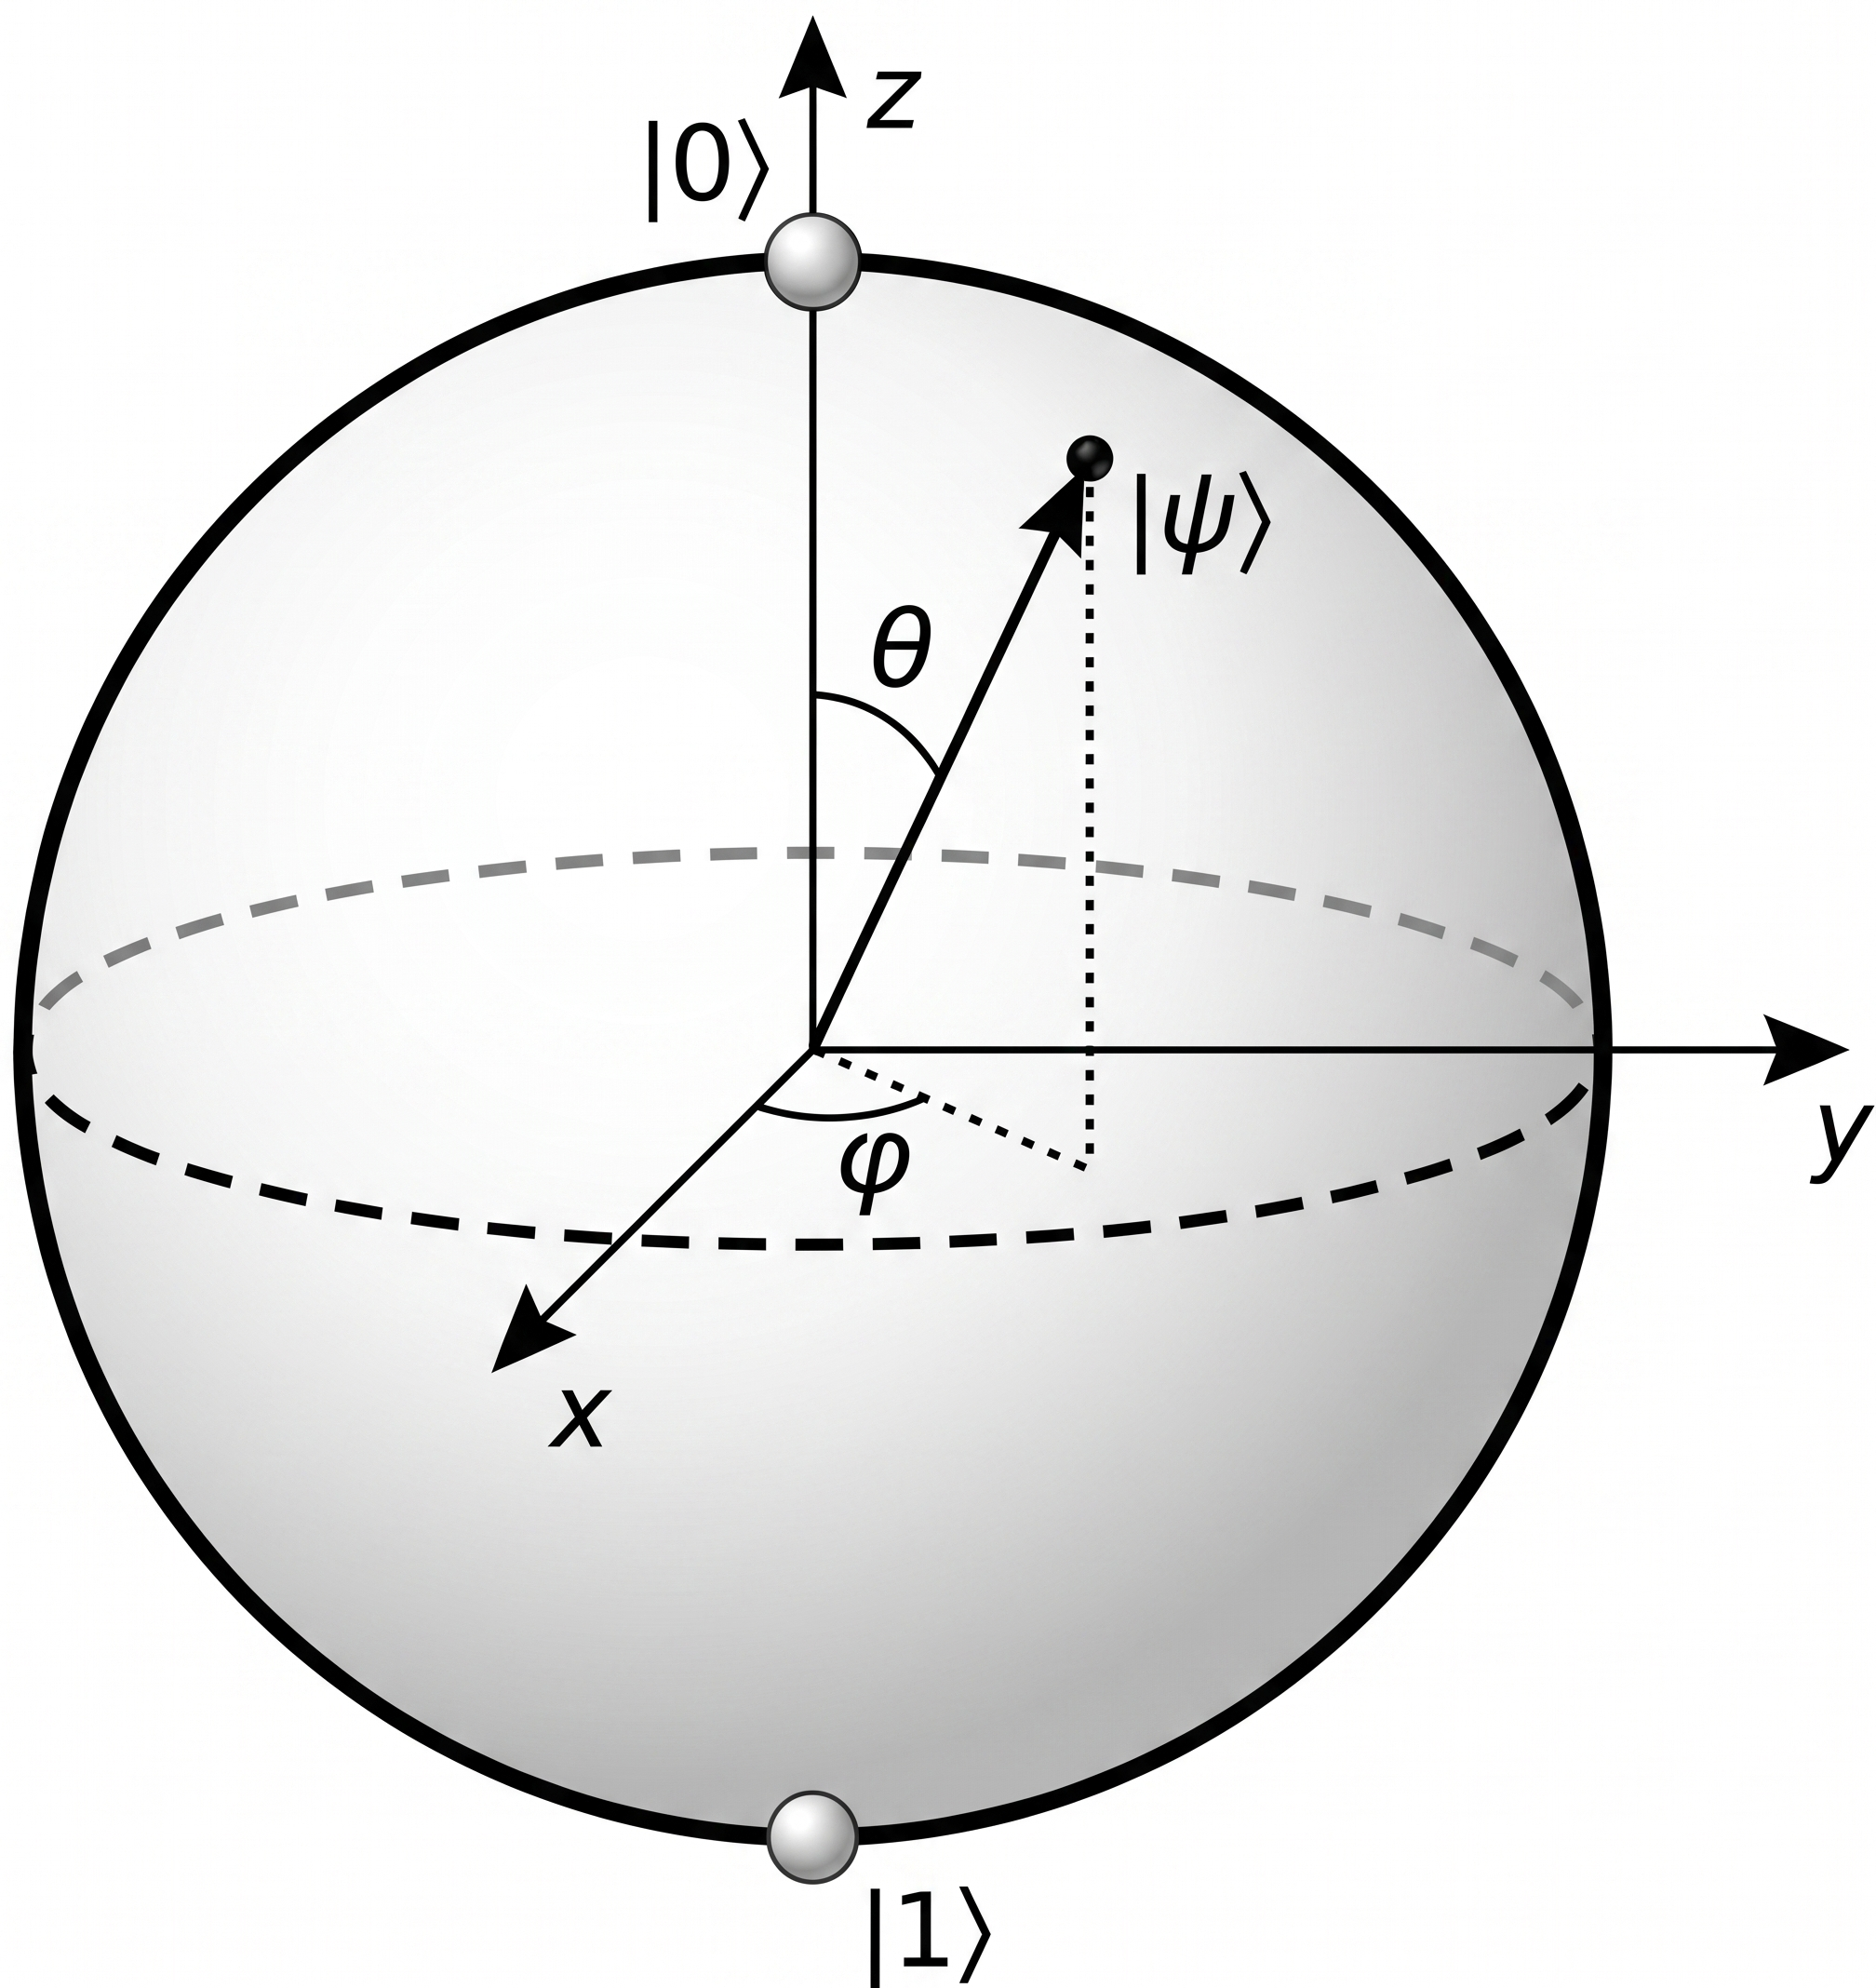
\includegraphics[width=0.5\textwidth]{assets/matcauBloch.png}
    \caption{Minh họa về mặt cầu Bloch.}
\end{figure}

Các điểm đặc biệt trên mặt cầu Bloch có thể được đọc trực tiếp từ phương trình
\eqref{eq:bloch-param} và dễ dàng xác định qua bảng sau:

\begin{table}[htbp]
\centering
\caption{Bảng trạng thái trên mặt cầu Bloch}
\renewcommand{\arraystretch}{1.4}
\begin{tabular}{lll}
\hline
Trạng thái & Tọa độ $(\theta, \phi)$ & Vị trí trên mặt cầu \\
\hline
$|0\rangle$ & $(0, \cdot)$ & Cực bắc \\
$|1\rangle$ & $(\pi, \cdot)$ & Cực nam \\
$|{+}\rangle$ & $(\pi/2, 0)$ & Xích đạo, hướng $+x$ \\
$|{-}\rangle$ & $(\pi/2, \pi)$ & Xích đạo, hướng $-x$ \\
$|{+i}\rangle = \frac{|0\rangle+i|1\rangle}{\sqrt{2}}$ & $(\pi/2, \pi/2)$ & Xích đạo, hướng $+y$\\
\hline
\end{tabular}
\label{tab:mat_cau_bloch}
\end{table}

\begin{remark}
Một đặc tính hình học quan trọng: hai trạng thái \emph{trực giao} về mặt đại số, tức là $\langle\phi|\psi\rangle = 0$ nhưng lại không vuông góc mà nằm ở \emph{hai cực
đối nhau} (\textit{antipodal}) trên mặt cầu Bloch. Chẳng hạn, $|0\rangle$ và
$|1\rangle$ nằm tại cực bắc và cực nam, còn $|+\rangle$ và $|-\rangle$ nằm đối
xứng qua tâm trên trục $x$. Điều này phản ánh thực tế rằng trong $\mathbb{C}^2$,
hai vectơ trực giao tạo thành góc $90°$ trong không gian Hilbert, nhưng biểu diễn
hình học trên mặt cầu Bloch bị ``kéo đôi" góc đó lên $180°$.
\end{remark}

Mặt cầu Bloch còn cung cấp diễn giải hình học tự nhiên cho các cổng lượng tử
đơn qubit. Có thể chứng minh rằng mọi toán tử unitary $U$ trên $\mathbb{C}^2$
đều có thể viết dưới dạng \cite{ref5}:
$$U = e^{-i\alpha\hat{n}\cdot\vec{\sigma}/2},$$
trong đó $\alpha \in \mathbb{R}$ là góc quay, $\hat{n}$ là vectơ đơn vị trong
$\mathbb{R}^3$ xác định trục quay, và $\vec{\sigma} = (\sigma_x, \sigma_y,
\sigma_z)$ là bộ ba ma trận $2\times 2$ được gọi là \textbf{ma trận Pauli} --
sẽ được định nghĩa tường minh ở mục 2.2. Biểu thức này có nghĩa là
mọi cổng lượng tử đơn qubit tương ứng với một \textbf{phép quay} vectơ Bloch
quanh trục $\hat{n}$ với góc $\alpha$ -- nhất quán với Tiên đề~2 rằng mọi tiến
hóa của hệ khép kín đều là unitary. Ví dụ đơn giản nhất: chọn $\hat{n} =
\hat{z}$ và $\alpha = \pi$, phép quay $180°$ quanh trục $z$ biến $|{+}\rangle$
tại xích đạo thành $|{-}\rangle$ -- giữ nguyên vĩ độ, đảo ngược kinh độ. Các
cổng cụ thể và phép quay Bloch tương ứng sẽ được phân tích đầy đủ ở mục 2.2.

% ---------------------------------------------------------------
\subsection*{Hệ nhiều qubit và tích tensor}

Khi mở rộng từ một qubit đơn lẻ sang hệ phức hợp, không gian trạng thái được
xây dựng bằng phép tích tensor (mục~\ref{subsec:tensor}) theo Tiên đề~4
(mục~\ref{sec:postulates}). Không gian trạng thái của hệ hai qubit là
$\mathbb{C}^2 \otimes \mathbb{C}^2$ -- không gian Hilbert bốn chiều với cơ sở
tính toán \cite{ref5}:
$$\{|00\rangle,\; |01\rangle,\; |10\rangle,\; |11\rangle\},$$
trong đó $|ab\rangle$ là ký hiệu tắt của $|a\rangle \otimes |b\rangle$.
Trạng thái tổng quát của hệ hai qubit là:
\begin{equation}
    |\psi\rangle = \alpha_{00}|00\rangle + \alpha_{01}|01\rangle
                + \alpha_{10}|10\rangle + \alpha_{11}|11\rangle,
    \quad \sum_{i,j}|\alpha_{ij}|^2 = 1.
    \label{eq:two-qubit}
\end{equation}

Tổng quát hóa lên hệ $n$ qubit, không gian trạng thái là $(\mathbb{C}^2)^{\otimes n}$
có số chiều $2^n$ -- tăng \emph{theo hàm mũ} với số qubit. Đây là nguồn gốc của
tính song song lượng tử: một trạng thái chồng chất đồng đều trên tất cả $2^n$ chuỗi
bit
\begin{equation}
    \frac{1}{\sqrt{2^n}}\sum_{x=0}^{2^n-1}|x\rangle
    \label{eq:uniform-superposition}
\end{equation}
mã hóa đồng thời $2^n$ giá trị đầu vào chỉ với $n$ qubit -- một bước khởi đầu trung
tâm trong thuật toán Deutsch--Jozsa.

\begin{example}[Trạng thái tích và trạng thái vướng víu]
Xét hai qubit, mỗi qubit ở trạng thái $|+\rangle = \frac{1}{\sqrt{2}}(|0\rangle
+ |1\rangle)$. Trạng thái của hệ là:
$$|{+}\rangle \otimes |{+}\rangle
= \frac{1}{2}(|00\rangle + |01\rangle + |10\rangle + |11\rangle).$$
Đây là \textbf{trạng thái tích} (\textit{product state}): có thể phân tách thành
tích của hai trạng thái qubit độc lập. Kết quả đo trên qubit thứ nhất không ảnh
hưởng đến phân bố xác suất của qubit thứ hai.

Ngược lại, trạng thái Bell
$$|\Phi^+\rangle = \frac{1}{\sqrt{2}}(|00\rangle + |11\rangle)$$
là \textbf{trạng thái vướng víu} (\textit{entangled state}): không thể viết dưới
dạng $|\psi_A\rangle \otimes |\psi_B\rangle$ cho bất kỳ $|\psi_A\rangle,
|\psi_B\rangle \in \mathbb{C}^2$ nào. Nếu đo qubit thứ nhất thu được $|0\rangle$,
qubit thứ hai lập tức suy sụp về $|0\rangle$ với xác suất $1$ -- bất kể khoảng
cách không gian giữa hai qubit.
\end{example}


\section{Cổng lượng tử một qubit và hai qubit}
\label{sec:gates}

Trong mô hình mạch lượng tử, sự tiến hóa của các trạng thái qubit được thực hiện thông qua các phép biến đổi tuyến tính bảo toàn chuẩn, gọi là \textbf{cổng lượng tử} (\textit{quantum gates}) \cite{ref5}. Khác với các cổng logic cổ điển như AND hay OR vốn không thuận nghịch, mọi cổng lượng tử đều được biểu diễn bằng một ma trận unitary và do đó luôn thuận nghịch. Cụ thể, cổng tác động lên hệ $n$ qubit được biểu diễn bằng một ma trận unitary kích thước $2^n \times 2^n$ thỏa mãn điều kiện $U^\dagger U = I$, trong đó $I$ là toán tử đồng nhất, và phép biến đổi ngược tương ứng với ma trận liên hợp Hermitian $U^\dagger$ của nó.

% ---------------------------------------------------------------
\subsection*{Ma trận Pauli và cổng Hadamard}

Bốn cổng một qubit cơ bản nhất là ma trận Pauli $X, Y, Z$ (hoặc $\sigma_1, \sigma_2, \sigma_3$) và cổng Hadamard $H$.
Cả bốn đều vừa là Hermitian vừa là unitary, tức $U^\dagger = U$ và $U^2 = I$
một tính chất đặc biệt không phải cổng nào cũng có \cite{ref5}.

\begin{definition}[Ma trận Pauli]
\label{def:pauli}
Ba \textbf{ma trận Pauli} là các toán tử một qubit được định nghĩa bởi:
$$X = \begin{pmatrix}0&1\\1&0\end{pmatrix}, \qquad
  Y = \begin{pmatrix}0&-i\\i&0\end{pmatrix}, \qquad
  Z = \begin{pmatrix}1&0\\0&-1\end{pmatrix}.$$
\end{definition}

\begin{proposition}[Tính chất đại số của ma trận Pauli]
\label{prop:pauli}
Các ma trận Pauli thỏa mãn:
\begin{enumerate}[label=(\roman*)]
    \item $X^2 = Y^2 = Z^2 = I$ \quad (tự nghịch đảo),
    \item $XY = iZ,\quad YZ = iX,\quad ZX = iY$ \quad (quan hệ giao hoán vòng),
    \item $XY = -YX,\quad YZ = -ZY,\quad ZX = -XZ$ \quad (phản giao hoán).
\end{enumerate}
\end{proposition}

Tác động của từng cổng Pauli lên cơ sở tính toán cho thấy vai trò hình học của
chúng trên mặt cầu Bloch \cite{ref5}:

\begin{example}[Tác động của các cổng Pauli]
\label{ex:pauli-action}
\textbf{Cổng $X$ -- lật bit lượng tử.} Cổng $X$ hoán vị hai trạng thái cơ sở:
$$X|0\rangle = |1\rangle, \qquad X|1\rangle = |0\rangle.$$
Với trạng thái tổng quát $|\psi\rangle = \alpha|0\rangle + \beta|1\rangle$:
$$X|\psi\rangle = \beta|0\rangle + \alpha|1\rangle.$$
Đây là phép quay góc $\pi$ quanh trục $x$ trên mặt cầu Bloch -- tương tự cổng
NOT cổ điển nhưng tác động lên biên độ phức.

\textbf{Cổng $Z$ -- lật pha.} Cổng $Z$ giữ nguyên $|0\rangle$ và đổi dấu $|1\rangle$:
$$Z|0\rangle = |0\rangle, \qquad Z|1\rangle = -|1\rangle.$$
Với trạng thái tổng quát:
$$Z|\psi\rangle = \alpha|0\rangle - \beta|1\rangle.$$
Không có tương đương cổ điển: $Z$ không thay đổi xác suất đo trong cơ sở tính
toán ($|\alpha|^2$ và $|\beta|^2$ giữ nguyên), nhưng thay đổi pha tương đối
và ảnh hưởng trực tiếp đến giao thoa. Trên mặt cầu
Bloch, đây là phép quay góc $\pi$ quanh trục $z$.

\textbf{Cổng $Y$.} Cổng $Y$ kết hợp cả lật bit lẫn lật pha:
$$Y|0\rangle = i|1\rangle, \qquad Y|1\rangle = -i|0\rangle,$$
tương ứng với phép quay góc $\pi$ quanh trục $y$ trên mặt cầu Bloch.
\end{example}

\begin{definition}[Cổng Hadamard]
\label{def:hadamard}
\textbf{Cổng Hadamard} $H$ được định nghĩa bởi:
$$H = \frac{1}{\sqrt{2}}\begin{pmatrix}1&1\\1&-1\end{pmatrix}.$$
\end{definition}

\begin{proposition}[Tính chất của cổng Hadamard]
\label{prop:hadamard}
Cổng Hadamard thỏa mãn $H^\dagger = H$ và $H^2 = I$. Tác động lên cơ sở tính
toán:
$$H|0\rangle = \frac{|0\rangle+|1\rangle}{\sqrt{2}} = |{+}\rangle, \qquad
  H|1\rangle = \frac{|0\rangle-|1\rangle}{\sqrt{2}} = |{-}\rangle,$$
và ngược lại $H|{+}\rangle = |0\rangle$, $H|{-}\rangle = |1\rangle$.
\end{proposition}

\begin{remark}
Cổng Hadamard là cổng trung tâm trong hầu hết các thuật toán lượng tử. Nó tạo ra
trạng thái chồng chất đồng đều từ trạng thái cơ sở -- bước khởi tạo bắt buộc
trong thuật toán Deutsch--Jozsa. Cụ thể, áp dụng $H^{\otimes n}$ lên
$|0\rangle^{\otimes n}$ tạo ra chồng chất đồng đều trên tất cả $2^n$ chuỗi bit, cho phép oracle $U_f$ xử lý toàn bộ đầu
vào trong một bước duy nhất (Khái niệm oracle $U_f$ sẽ được định nghĩa ở cuối mục 3.1 thuộc chương 3). Trên mặt cầu Bloch, $H$ tương ứng với phép quay góc
$\pi$ quanh trục $\hat{n} = \frac{1}{\sqrt{2}}(\hat{x}+\hat{z})$, biến cực bắc
$|0\rangle$ thành điểm xích đạo $|+\rangle$.
\end{remark}

% ---------------------------------------------------------------
\subsection*{Cổng pha $S$ và $T$}

Ngoài các cổng Pauli và Hadamard, hai cổng pha thường gặp trong tính toán lượng
tử là $S$ và $T$ \cite{ref5}:
$$S = \begin{pmatrix}1&0\\0&i\end{pmatrix}, \qquad
  T = \begin{pmatrix}1&0\\0&e^{i\pi/4}\end{pmatrix}.$$

\begin{remark}
Cả hai cổng đều giữ nguyên $|0\rangle$ và thêm một pha tương đối vào $|1\rangle$:
$S|1\rangle = i|1\rangle$ (quay góc $\frac{\pi}{2}$ quanh trục $z$) và
$T|1\rangle = e^{i\pi/4}|1\rangle$ (quay góc $\frac{\pi}{4}$ quanh trục $z$). Cần lưu ý
rằng $S = T^2$ và $Z = S^2 = T^4$, tức $Z$, $S$, $T$ là các phép quay quanh
cùng trục $z$ với góc lần lượt là $\pi$, $\frac{\pi}{2}$, $\frac{\pi}{4}$. Hai cổng này không
xuất hiện trực tiếp trong thuật toán Deutsch--Jozsa nhưng là thành phần cốt lõi
của bộ cổng phổ dụng được đề cập ở cuối mục này.
\end{remark}

% ---------------------------------------------------------------
\subsection*{Cổng CNOT, Toffoli và tính phổ dụng}

Các cổng một qubit không đủ để tạo ra sự vướng víu -- đặc tính phi cổ điển đòi
hỏi tương tác giữa nhiều qubit. Cổng hai qubit cơ bản nhất là
\textbf{CNOT} (\textit{Controlled-NOT}) \cite{ref5}.

\begin{definition}[Cổng CNOT]
\label{def:cnot}
Cổng \textbf{CNOT} tác động lên không gian $\mathbb{C}^2 \otimes \mathbb{C}^2$
với hai qubit đóng vai trò \emph{điều khiển} (\textit{control}) và \emph{đích}
(\textit{target}):
$$\mathrm{CNOT} =
\begin{pmatrix}1&0&0&0\\0&1&0&0\\0&0&0&1\\0&0&1&0\end{pmatrix},$$
tác động lên cơ sở tính toán theo quy tắc
$|c\rangle|t\rangle \mapsto |c\rangle|t \oplus c\rangle$,
trong đó $\oplus$ là phép cộng modulo $2$.
\end{definition}

\begin{example}[Tạo trạng thái Bell bằng CNOT]
\label{ex:bell}
Áp dụng $H$ lên qubit điều khiển rồi tác dụng CNOT:
$$|00\rangle \xrightarrow{H \otimes I}
  \frac{|0\rangle+|1\rangle}{\sqrt{2}}|0\rangle
  \xrightarrow{\mathrm{CNOT}}
  \frac{|00\rangle+|11\rangle}{\sqrt{2}} = |\Phi^+\rangle.$$
Trạng thái Bell $|\Phi^+\rangle$ là trạng thái vướng víu -- không thể phân tách
thành tích của hai trạng thái qubit độc lập (xem mục~\ref{sec:qubit}).
\end{example}

\begin{definition}[Cổng Toffoli]
\label{def:toffoli}
Cổng \textbf{Toffoli} (hay \textbf{CCNOT}) tác động lên không gian
$(\mathbb{C}^2)^{\otimes 3}$ với hai qubit điều khiển $c_1$, $c_2$ và một qubit
đích $t$:
$$\mathrm{Toffoli} =
\begin{pmatrix}
1&0&0&0&0&0&0&0\\
0&1&0&0&0&0&0&0\\
0&0&1&0&0&0&0&0\\
0&0&0&1&0&0&0&0\\
0&0&0&0&1&0&0&0\\
0&0&0&0&0&1&0&0\\
0&0&0&0&0&0&0&1\\
0&0&0&0&0&0&1&0
\end{pmatrix},$$
tác động lên cơ sở tính toán theo quy tắc
$$|c_1\rangle|c_2\rangle|t\rangle
  \mapsto |c_1\rangle|c_2\rangle|t \oplus (c_1 \wedge c_2)\rangle,$$
trong đó $\wedge$ là phép AND logic. Qubit đích bị lật khi và chỉ khi
\emph{cả hai} qubit điều khiển đều ở trạng thái $|1\rangle$; trong mọi trường
hợp còn lại, toàn bộ hệ giữ nguyên.
\end{definition}

\begin{remark}
Cổng Toffoli có ý nghĩa lý thuyết quan trọng vì quy tắc
$t \mapsto t \oplus (c_1 \wedge c_2)$ mô phỏng cổng AND cổ điển trong môi trường
\emph{khả nghịch}: chọn $t = 0$ thì qubit đích sau phép biến đổi chứa đúng giá
trị $c_1 \wedge c_2$, trong khi hai qubit điều khiển được bảo toàn nguyên vẹn.
Điều này là cơ sở để chứng minh mọi phép tính cổ điển đều có thể được mô phỏng
trên máy tính lượng tử.

Về \textbf{tính phổ dụng} (\textit{universality}): một bộ cổng được gọi là phổ
dụng nếu mọi toán tử unitary đều có thể xấp xỉ tùy ý chính xác bằng tổ hợp hữu
hạn các cổng trong bộ đó \cite{ref5}. Bộ $\{H, T, \mathrm{CNOT}\}$ là một bộ
cổng phổ dụng -- mọi thuật toán lượng tử đều có thể biên dịch về ba cổng này.
Đây là lý do $H$ và $T$ xuất hiện trong hầu hết các phân tích độ phức tạp mạch,
trong khi thuật toán Deutsch--Jozsa chỉ cần $H$ và $\mathrm{CNOT}$ (ẩn trong
cấu trúc oracle $U_f$) là đủ.
\end{remark}

\section{Mạch lượng tử: cấu trúc và phép đo}
\label{sec:circuit-measure}

Các cổng lượng tử đơn thuần mô tả từng phép biến đổi đơn lẻ. Để
thực hiện một thuật toán, các cổng đó cần được sắp xếp theo một trình tự xác định, đây là vai trò của \textbf{mạch lượng tử} (\textit{quantum circuit}). Mục này
trình bày cách đọc và phân tích mạch lượng tử, cơ chế phép đo kết thúc mạch, và
các tiêu chí đánh giá độ phức tạp -- ba công cụ cần thiết để theo dõi phân tích
thuật toán Deutsch--Jozsa.

% ---------------------------------------------------------------
\subsection*{Biểu đồ mạch và quy ước ký hiệu}

\begin{definition}[Mạch lượng tử]
\label{def:circuit}
Một \textbf{mạch lượng tử} trên $n$ qubit là một dãy hữu hạn các cổng lượng tử
$G_1, G_2, \dots, G_d$ tác động lần lượt lên các qubit của thanh ghi, kết thúc
bởi một hoặc nhiều phép đo \cite{ref5}. Toán tử unitary của toàn mạch là tích
có thứ tự:
$$U_{\mathrm{circuit}} = G_d \cdots G_2 G_1.$$
\end{definition}

Biểu đồ mạch là cách trực quan hóa định nghĩa trên theo quy ước sau \cite{ref5}:

\begin{convention}[Ký hiệu biểu đồ mạch]
\label{conv:circuit}
\hfill
\begin{enumerate}[label=(\roman*)]
    \item Mỗi \textbf{đường ngang} (dây) biểu diễn một qubit, thời gian chạy
          từ trái sang phải.
    \item Mỗi \textbf{hộp} trên dây biểu diễn một cổng, ký hiệu bằng tên cổng
          ($H$, $X$, $Z$, \ldots).
    \item \textbf{Cổng điều khiển} được ký hiệu bằng một điểm đặc $\bullet$ trên
          dây điều khiển, nối bằng đường thẳng đứng xuống cổng đích.
    \item \textbf{Phép đo} được ký hiệu bằng biểu tượng đồng hồ đo ở
          cuối dây, kèm đường đôi dẫn ra kết quả cổ điển.
    \item Trạng thái đầu vào của qubit thứ $k$ được ghi ở đầu dây tương ứng,
          thường là $|0\rangle$.
\end{enumerate}
Hình ảnh trực quan về ký hiệu mạch và dạng ma trận của các cổng lượng tử được trình bày ở Phụ lục 2.
\end{convention}

\begin{example}[Mạch tạo trạng thái Bell]
\label{ex:bell-circuit}
Mạch tạo trạng thái Bell $|\Phi^+\rangle$ được biểu diễn
như sau:


\begin{figure}[H]
    \centering
    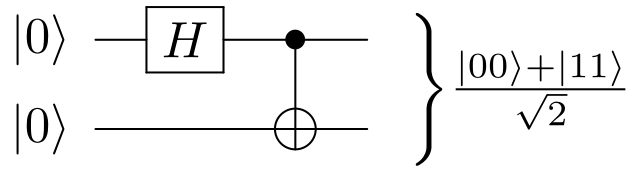
\includegraphics[width=0.8\textwidth]{assets/Bell-state.png}
    \caption{Mạch tạo trạng thái Bell.}
    \vspace{0.2cm}
    \small\textit{Nguồn: Wikipedia.}
\end{figure}

Đọc từ trái sang phải: cổng $H$ tác động lên qubit thứ nhất tạo trạng thái
$|+\rangle$, sau đó cổng CNOT với qubit thứ nhất làm điều khiển và qubit thứ
hai làm đích tạo ra vướng víu, cho kết quả
$|\Phi^+\rangle = \frac{1}{\sqrt{2}}(|00\rangle + |11\rangle)$.
\end{example}

\begin{remark}
Thứ tự nhân ma trận \emph{ngược} với thứ tự đọc trên biểu đồ: cổng xuất hiện
đầu tiên (trái nhất) trong biểu đồ tương ứng với toán tử đứng \emph{phải nhất}
trong tích ma trận. Trong Ví dụ~\ref{ex:bell-circuit}, toán tử toàn mạch là
$U = \mathrm{CNOT} \cdot (H \otimes I)$, không phải $(H \otimes I) \cdot
\mathrm{CNOT}$.
\end{remark}

% ---------------------------------------------------------------
\subsection*{Phép đo và sụp đổ trạng thái}

Phép đo kết thúc mạch lượng tử là ứng dụng trực tiếp của Tiên đề~3
(mục~\ref{sec:postulates}) vào thanh ghi qubit. Trong thực tế tính toán lượng
tử, phép đo hầu như luôn được thực hiện trong \textbf{cơ sở tính toán}
$\{|0\rangle, |1\rangle\}^{\otimes n}$ \cite{ref5}.

\begin{figure}[H]
    \centering
    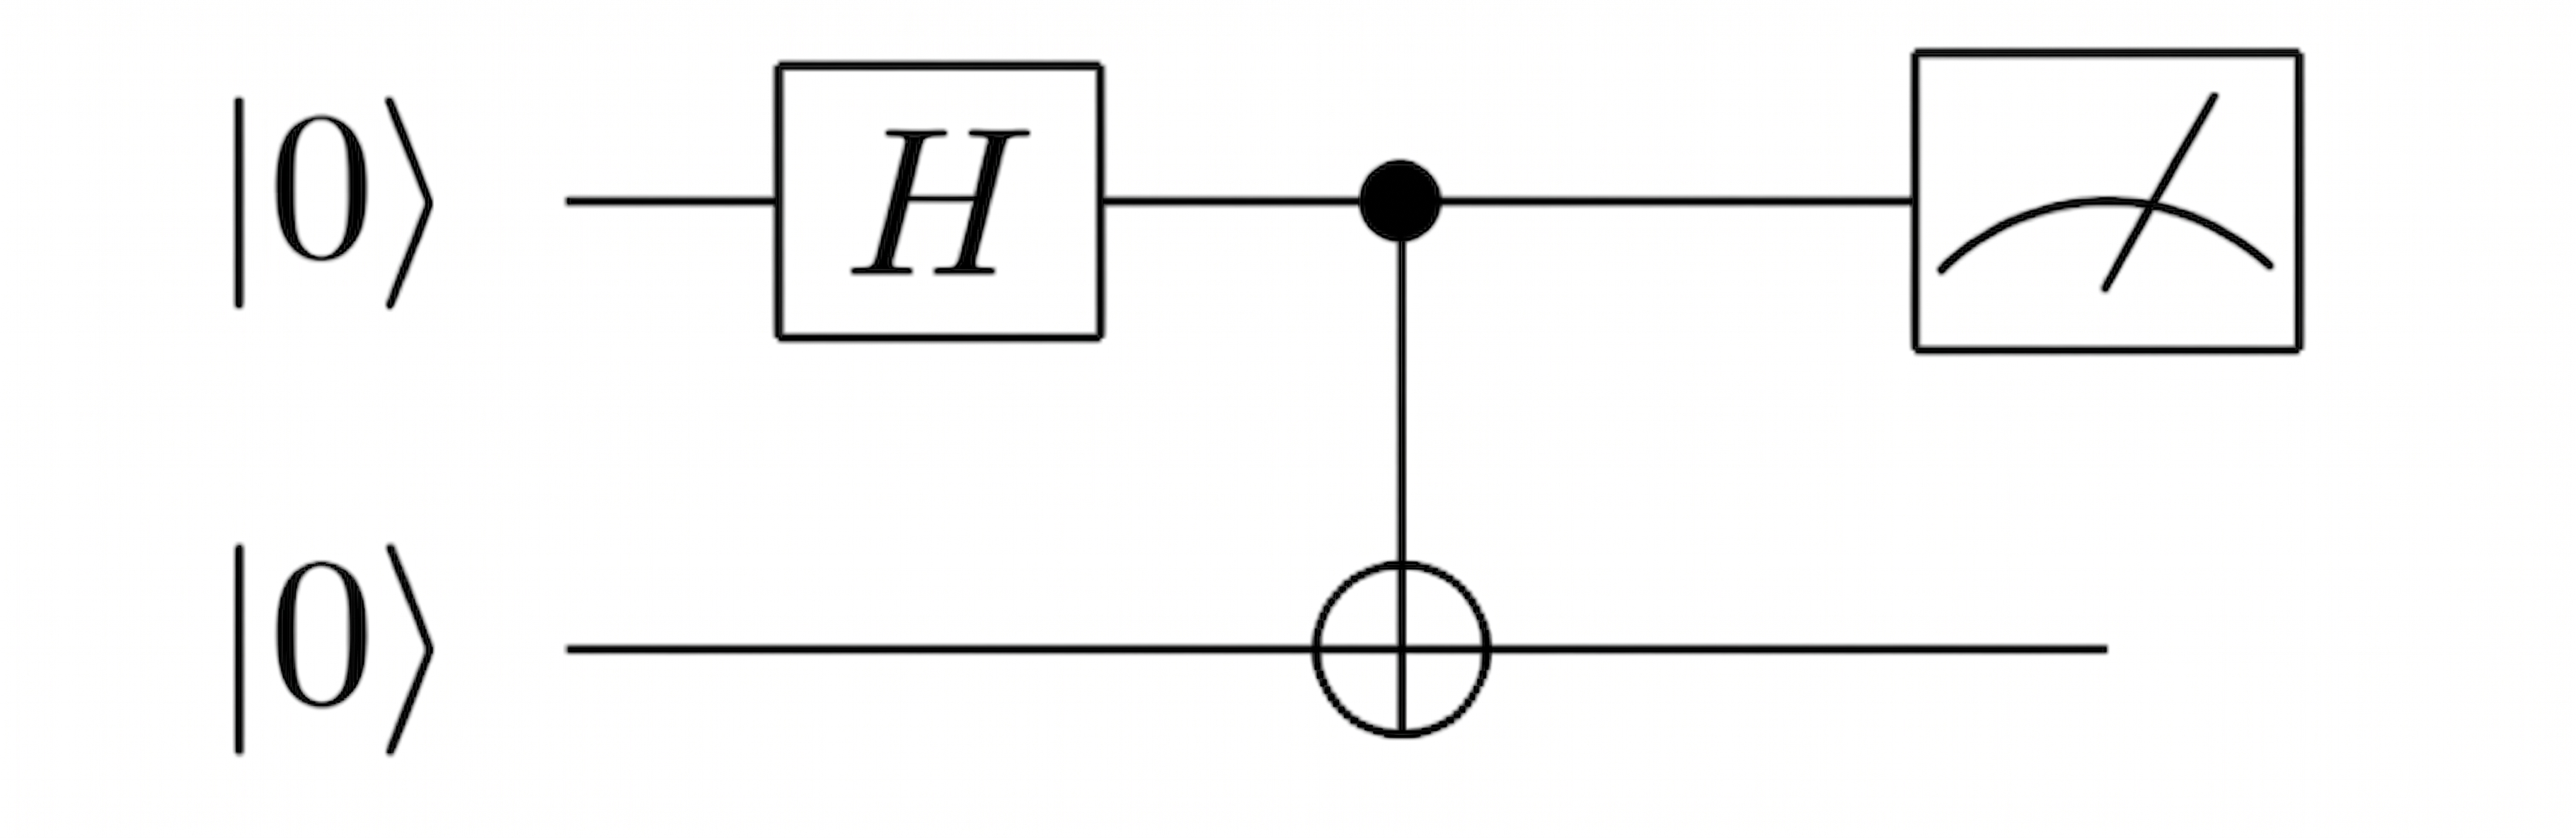
\includegraphics[width=0.8\textwidth]{assets/phepdo.png}
    \caption{Phép đo cho mạch tạo trạng thái Bell.}
\end{figure}

\begin{proposition}[Phép đo trong cơ sở tính toán]
\label{prop:measurement}
Cho hệ $n$ qubit ở trạng thái
$|\psi\rangle = \sum_{x \in \{0,1\}^n} \alpha_x |x\rangle$
với $\sum_x |\alpha_x|^2 = 1$. Khi đo toàn bộ thanh ghi trong cơ sở tính toán:
\begin{enumerate}[label=(\roman*)]
    \item Kết quả thu được là chuỗi bit $x \in \{0,1\}^n$ với xác suất
          $p(x) = |\alpha_x|^2$.
    \item Sau phép đo, trạng thái sụp đổ về $|x\rangle$ -- mọi thông tin về
          các biên độ khác bị xóa bỏ không thể phục hồi.
\end{enumerate}
\end{proposition}

\begin{remark}
Tính không khả nghịch của phép đo là điểm mấu chốt phân biệt mạch lượng tử với
các phép biến đổi unitary: trong khi mỗi cổng $U$ có thể đảo ngược bằng $U^\dagger$,
phép đo phá hủy thông tin về chồng chất và không có thao tác nào khôi phục lại
trạng thái trước đo. Vì lý do này, trong thiết kế mạch, phép đo \emph{luôn được
đặt ở cuối} sau tất cả các cổng unitary -- trừ các trường hợp đặc biệt như đo
giữa chừng trong tính toán có điều kiện.
\end{remark}


% ---------------------------------------------------------------
\subsection*{Độ phức tạp mạch: chiều sâu và số cổng}

Để so sánh hiệu quả của các thuật toán lượng tử, cần có tiêu chí định lượng mô
tả tài nguyên mà một mạch tiêu thụ. Hai tiêu chí phổ biến nhất là số cổng và
chiều sâu mạch \cite{ref5}.

\begin{definition}[Số cổng và chiều sâu mạch]
\label{def:complexity}
Cho mạch lượng tử $\mathcal{C}$:
\begin{enumerate}[label=(\roman*)]
    \item \textbf{Số cổng} (\textit{gate count}) là tổng số cổng trong mạch,
          đo lường tài nguyên tính toán tổng thể.
    \item \textbf{Chiều sâu} (\textit{circuit depth}) là số lớp cổng tối thiểu
          khi sắp xếp các cổng không tác động lên cùng qubit vào cùng một lớp --
          đo lường thời gian thực thi song song.
\end{enumerate}
\end{definition}

\begin{example}[Số cổng và chiều sâu của mạch Bell]
\label{ex:bell-complexity}
Mạch tạo trạng thái Bell ở Ví dụ~\ref{ex:bell-circuit} có:
\begin{itemize}
    \item Số cổng: $2$ (một cổng $H$ và một cổng CNOT).
    \item Chiều sâu: $2$ (cổng $H$ và CNOT không thể thực hiện song song vì
          CNOT phụ thuộc vào đầu ra của $H$).
\end{itemize}
\end{example}

\subsection*{Kết luận cuối Chương 2}
Chương này đã triển khai nền tảng toán học của Chương~1 thành mô hình
tính toán lượng tử cụ thể. Qubit được xác định là đơn vị thông tin cơ bản
với biểu diễn hình học trực quan trên mặt cầu Bloch; các cổng lượng tử
Pauli, Hadamard và CNOT được phân tích như các toán tử unitary tác động
lên trạng thái qubit; cấu trúc mạch và tiêu chí độ phức tạp cung cấp
ngôn ngữ để mô tả và đánh giá thuật toán.